\chapter{Organization Essence Revealing}

The goals of this chapter are to perform an OER analysis as described in~\cite{dietz2015teoo,dietz2020enterprise}. For simplicity, we will only do the following steps: 

\begin{enumerate}
    \item Insert the project domain description into this document. 
    \item Perform the OER analysis and find \oact{ontological acts}. Be vigilant about the \btrap{blue traps}!
    \item Identify ontological transaction kinds and put them in the text. E.g. \oact{[TK1/rq]} If there are not enough red transactions, you can include the green ones. 
    \item Create an extended transaction result table (e-TRT). Map the transaction acts to the project domain description. See the~\cref{tab:etrt}. 
    \item Create a Subject-Actor table to realize the distinction between roles and DEMO actor roles. See the~\cref{tab:subjectactortable}. 
    \item Think in trees, not in flows and create the interaction structure of your transaction kinds. See the~\cref{fig:interactionStructure}.  
    \item Produce the Coordination Structure Diagram (CSD) and the Object Fact Diagram (OFD). See the~\cref{fig:csdModel} and ~\cref{fig:ofdModel}.  
    \item Finally, summarize your modeling thoughts and revelations. Don't forget about missing transaction steps table~\cref{tab:missing_transaction_steps}. 
\end{enumerate}

The process description of the Volley Case and it's OER analysis was taken from the Enterprise Ontology book~\cite{dietz2020enterprise}. 

%In the step 1 a coloring of the process description is made. The coloring can be done on text as well as on the flow chart diagram. 
\section{OER Step 1: Distinguishing Performa-Informa-Forma}

Legend: 
\begin{itemize}
    \item \oact{Ontological Act [Transaction Kind/Act type]}
    \item \btrap{Blue trap ontological act}!
\end{itemize}

\textbf{\Large Hlava čtvrtá}

\textbf{\Large Rozhodnutí}

\textbf{\Large Rozsudek}

\paragraph{\S 152}

\begin{enumerate}[label={(\arabic*)}]
\item Rozsudkem rozhoduje soud o věci samé. Zákon stanoví, kdy soud rozhoduje ve věci samé usnesením. 
\item Rozsudkem má být rozhodnuto o celé projednávané věci. Jestliže to však je účelné, může soud rozsudkem rozhodnout nejdříve jen o její části nebo jen o jejím základu.
\end{enumerate}

\paragraph{\S 153}

\begin{enumerate}[label={(\arabic*)}]
  \item Soud rozhoduje na základě zjištěného skutkového stavu věci.
  \item Soud může překročit návrhy účastníků a přisoudit něco jiného nebo více, než čeho se domáhají, jen tehdy, jestliže z právního předpisu vyplývá určitý způsob vypořádání vztahu mezi účastníky.
\end{enumerate}

\paragraph{\S 153a}

\begin{enumerate}[label={(\arabic*)}]
  \item \oact{Uzná-li žalovaný v průběhu soudního řízení nárok [TK1/rq]} nebo základ nároku, který je proti němu žalobou uplatňován, \oact{rozhodne soud rozsudkem podle tohoto uznání [TK1/da]}. Uzná-li žalovaný nárok proti němu žalobou uplatněný jen zčásti, rozhodne soud rozsudkem podle tohoto uznání, jen navrhne-li to žalobce.
  \item \oact{Rozsudek pro uznání nelze vydat ve věcech, v nichž nelze uzavřít a schválit smír [TK1/dc]} (§ 99 odst. 1 a 2).
  \item Rozsudkem pro uznání rozhodne soud také tehdy, má-li se za to, že žalovaný nárok, který je proti němu žalobou uplatňován, uznal (§ 114b odst. 5 a § 114c odst. 6).
  \item Jen pro vydání rozsudku pro uznání nemusí být nařízeno jednání.
\end{enumerate}

\paragraph{\S 153b}

\begin{enumerate}[label={(\arabic*)}]
  \item Zmešká-li žalovaný, kterému byly \btrap{řádně doručeny} do jeho vlastních rukou (§ 49) žaloba a předvolání k jednání nejméně deset dnů přede dnem, kdy se jednání má konat, a který byl o následcích nedostavení se poučen, bez důvodné a včasné omluvy první jednání, které se ve věci konalo, a \oact{navrhne-li to žalobce [TK2/rq]}, který se dostavil k jednání, pokládají se tvrzení žalobce obsažená v žalobě o skutkových okolnostech, týkající se sporu, za nesporná a na tomto základě může \oact{soud rozhodnout o žalobě rozsudkem pro zmeškání. [TK2/da]}
  \item Je-li v jedné věci několik žalovaných, kteří mají takové společné povinnosti, že se rozsudek musí vztahovat na všechny (§ 91 odst. 2), \oact{lze rozhodnout rozsudkem pro zmeškání jen tehdy, nedostaví-li se k jednání všichni řádně obeslaní žalovaní.[TK2/dc]}
  \item \oact{Rozsudek pro zmeškání nelze vydat ve věcech, v nichž nelze uzavřít a schválit smír (§ 99 odst. 1 a 2), nebo došlo-li by takovým rozsudkem ke vzniku, změně nebo zrušení právního poměru mezi účastníky. [TK2/dc]}
  \item Zmešká-li žalovaný z omluvitelných důvodů první jednání ve věci, při němž byl vynesen rozsudek pro zmeškání, soud \oact{na návrh žalovaného [TK3/rq]} tento rozsudek \oact{usnesením zruší a nařídí jednání [TK3/da]}. Takový \oact{návrh může účastník podat nejpozději do dne právní moci rozsudku pro zmeškání. [TK3/dc]}
  \item Pokud žalovaný kromě návrhu na zrušení rozsudku soudu prvního stupně z důvodů podle odstavce 4 \oact{podal proti rozsudku i odvolání [T3/rj]} a \oact{návrhu na zrušení rozsudku bylo pravomocným usnesením vyhověno [T3/sp]}, k odvolání se nepřihlíží.
\end{enumerate}

\paragraph{\S 154}

\begin{enumerate}[label={(\arabic*)}]
  \item Pro rozsudek je rozhodující stav v době jeho vyhlášení.
  \item Jde-li o opětující se dávky, lze uložit povinnost i k plnění dávek, které se stanou splatnými teprve v budoucnu.
\end{enumerate}

\paragraph{\S 155}

\begin{enumerate}[label={(\arabic*)}]
  \item Obsah rozhodnutí ve věci samé vysloví soud ve výroku rozsudku. Ve výroku také rozhodne o povinnosti k náhradě nákladů řízení; rozhodne-li jen o základu náhrady nákladů řízení, určí její výši v samostatném usnesení.
  \item Výrok rozsudku o plnění v penězích může být vyjádřen v cizí měně, neodporuje-li to okolnostem případu a jestliže
  \begin{enumerate}[label={\alph*)}]
    \item plnění vychází z právního jednání, v němž je vyjádřeno v cizí měně, žalobce (navrhovatel) požaduje plnění v cizí měně a devizové předpisy umožňují tuzemci, který má plnit, plnění v navrhované cizí měně poskytnout bez zvláštního povolení, nebo
    \item některý z účastníků je cizozemcem.
  \end{enumerate}
  \item Nejsou-li splněny předpoklady pro přiznání plnění v cizí měně uvedené v odstavci 2, soud stanoví i bez návrhu plnění v měně České republiky.
  \item Ve věcech ochrany práv porušených nebo ohrožených nekalým soutěžním jednáním,ochrany práv z duševního vlastnictví a ve věcech ochrany práv spotřebitelů může soud účastníkovi, jehož žalobě vyhověl, přiznat na jeho návrh ve výroku rozsudku právo rozsudek uveřejnit na náklady neúspěšného účastníka; podle okolností případu soud stanoví též rozsah, formu a způsob uveřejnění.
\end{enumerate}

\paragraph{\S 156}

\begin{enumerate}[label={(\arabic*)}]
  \item Rozsudek se vyhlašuje vždy veřejně; vyhlašuje jej předseda senátu jménem republiky. Uvede přitom výrok rozsudku spolu s odůvodněním a poučením o odvolání a o možnosti výkonu rozhodnutí. Není-li přítomen vyhlášení rozsudku žádný z účastníků, uvede pouze výrok. Po vyhlášení předseda senátu zpravidla účastníky vyzve, aby se vyjádřili, zda se vzdávají odvolání proti vyhlášenému rozsudku.
  \item Rozsudek se vyhlašuje zpravidla hned po skončení jednání, které rozsudku předcházelo; není-li to možné, soud k vyhlášení rozsudku odročí jednání nejdéle na dobu deseti kalendářních dnů. Ustanovení § 119 odst. 2 a 3 se v tomto případě nepoužijí.
  \item Jakmile soud vyhlásí rozsudek, je jím vázán.
\end{enumerate}

\paragraph{\S 157}

\begin{enumerate}[label={(\arabic*)}]
  \item Není-li stanoveno jinak, v písemném vyhotovení rozsudku se po slovech "Jménem republiky" uvede označení soudu, jména a příjmení soudců a přísedících, přesné označení účastníků a jejich zástupců, účast státního zastupitelství a Úřadu pro zastupování státu ve věcech majetkových, označení projednávané věci, znění výroku, odůvodnění, poučení o tom, zda je přípustný opravný prostředek nepočítaje v to žalobu na obnovu řízení a pro zmatečnost, a o lhůtě a místu k jeho podání, poučení o možnosti výkonu rozhodnutí a den a místo vyhlášení. Je-li to možné, uvede se v označení účastníků též jejich datum narození (identifikační číslo).
  \item Není-li dále stanoveno jinak, soud v odůvodnění rozsudku uvede, čeho se žalobce (navrhovatel) domáhal a z jakých důvodů a jak se ve věci vyjádřil žalovaný (jiný účastník řízení), stručně a jasně vyloží, které skutečnosti má prokázány a které nikoliv, o které důkazy opřel svá skutková zjištění a jakými úvahami se při hodnocení důkazů řídil, proč neprovedl i další důkazy, jaký učinil závěr o skutkovém stavu a jak věc posoudil po právní stránce; není přípustné ze spisu opisovat skutkové přednesy účastníků a provedené důkazy. Soud dbá o to, aby odůvodnění rozsudku bylo přesvědčivé. Odůvodnění uvedené v písemném vyhotovení rozsudku musí být v souladu s vyhlášeným odůvodněním.
  \item V odůvodnění rozsudku pro uznání nebo rozsudku pro zmeškání uvede soud pouze předmět řízení a stručně vyloží důvody, pro které rozhodl rozsudkem pro uznání nebo rozsudkem pro zmeškání.
  \item V odůvodnění rozsudku, proti němuž není odvolání přípustné nebo proti němuž se účastníci odvolání vzdali (§ 207 odst. 1), soud uvede pouze předmět řízení, závěr o skutkovém stavu a stručné právní posouzení věci.
\end{enumerate}

\paragraph{\S 158}

\begin{enumerate}[label={(\arabic*)}]
  \item Písemné nebo elektronické vyhotovení rozsudku podepisuje předseda senátu. Nemůže-li je podepsat, podepíše je jiný člen senátu, a rozhodl-li samosoudce, jiný předsedou soudu pověřený soudce; důvod se na písemném vyhotovení poznamená. Rozsudek se vyhotovuje v té podobě, v jaké je veden spis.
  \item Stejnopis rozsudku vyhotoveného v listinné podobě a rozsudek vyhotovený v elektronické podobě se doručuje účastníkům, popřípadě jejich zástupcům do vlastních rukou.
  \item Jestliže se účastníci vzdali odvolání po skončení jednání, které rozsudku předcházelo, doručí se stejnopis vyhotovení rozsudku zpravidla při skončení jednání.
  \item Jestliže stejnopis vyhotovení rozsudku nebyl doručen podle odstavce 3, je třeba jej účastníkům, popřípadě jejich zástupcům odeslat ve lhůtě třiceti dnů ode dne vyhlášení rozsudku. Předseda soudu je oprávněn tuto lhůtu prodloužit až o dalších šedesát dnů.
\end{enumerate}

\paragraph{\S 159}

Doručený rozsudek, který již nelze napadnout odvoláním, je v právní moci.

\paragraph{\S 159a}

\begin{enumerate}[label={(\arabic*)}]
  \item Nestanoví-li zákon jinak, je výrok pravomocného rozsudku závazný jen pro účastníky řízení.
  \item Výrok pravomocného rozsudku, kterým bylo rozhodnuto ve věcech uvedených v § 83 odst. 2, je závazný nejen pro účastníky řízení, ale i pro další osoby oprávněné proti žalovanému pro tytéž nároky z téhož jednání nebo stavu. Zvláštní právní předpisy stanoví, v kterých dalších případech a v jakém rozsahu je výrok pravomocného rozsudku závazný pro jiné osoby než účastníky řízení.
  \item V rozsahu, v jakém je výrok pravomocného rozsudku závazný pro účastníky řízení a popřípadě jiné osoby, je závazný též pro všechny orgány.
  \item Jakmile bylo o věci pravomocně rozhodnuto, nemůže být v rozsahu závaznosti výroku rozsudku pro účastníky a popřípadě jiné osoby věc projednávána znovu.
\end{enumerate}

\paragraph{\S 160}

\begin{enumerate}[label={(\arabic*)}]
  \item Uložil-li soud v rozsudku povinnost, je třeba ji splnit do tří dnů od právní moci rozsudku nebo, jde-li o vyklizení bytu, do patnácti dnů od právní moci rozsudku; soud může určit lhůtu delší nebo stanovit, že peněžité plnění se může stát ve splátkách, jejichž výši a podmínky splatnosti určí.
  \item Odsoudil-li soud k opětujícímu se plnění v budoucnu splatných dávek, je třeba je plnit, jakmile se podle rozsudku stanou splatnými.
  \item Uložil-li soud pravomocným rozsudkem povinnost vyklidit obydlí až po zajištění náhradního bydlení, běží lhůta k vyklizení až ode dne zajištění náhradního bydlení.
  \item U rozsudků předběžně vykonatelných soud určí lhůtu k plnění od jejich doručení tomu, kdo má plnit.
\end{enumerate}

\paragraph{\S 161}

\begin{enumerate}[label={(\arabic*)}]
  \item Rozsudek je vykonatelný, jakmile uplyne lhůta k plnění.
  \item Není-li v rozsudku uložena povinnost k plnění, je rozsudek vykonatelný, jakmile nabyl právní moci.
  \item Pravomocné rozsudky ukládající prohlášení vůle nahrazují toto prohlášení.
\end{enumerate}

\paragraph{\S 162}

\begin{enumerate}[label={(\arabic*)}]
  \item Předběžně vykonatelné jsou rozsudky odsuzující k plnění výživného nebo pracovní odměny za poslední 3 měsíce před vyhlášením rozsudku.
  \item Na návrh může soud předběžnou vykonatelnost rozsudku vyslovit, a to ve výroku rozsudku, jestliže by jinak účastníku hrozilo nebezpečí těžko nahraditelné nebo značné újmy.
\end{enumerate}

\paragraph{\S 163}

Rozsudek odsuzující k plnění v budoucnu splatných dávek nebo k plnění ve splátkách je možno na návrh změnit, jestliže se podstatně změnily okolnosti, které jsou rozhodující pro výši a další trvání dávek nebo splátek. Nestanoví-li zákon jinak, je změna rozsudku přípustná od doby, kdy došlo ke změně poměrů.

\paragraph{\S 164}

Předseda senátu opraví v rozsudku kdykoliv i bez návrhu chyby v psaní a v počtech, jakož i jiné zjevné nesprávnosti. Týká-li se oprava výroku rozhodnutí nebo není-li možné provést opravu ve stejnopisech rozhodnutí, vydá o tom opravné usnesení, které doručí účastníkům; jde-li o opravu výroku rozhodnutí, může odložit vykonatelnost rozsudku na dobu, dokud opravné usnesení nenabude právní moci.

\paragraph{\S 165}

\begin{enumerate}[label={(\arabic*)}]
  \item \oact{Pokud odůvodnění rozsudku nemá podklad ve zjištění skutkového stavu, může účastník před tím, než rozsudek nabude právní moci, navrhnout, aby odůvodnění bylo opraveno. [TK4/rq]}
  \item \oact{Nevyhoví-li soud prvního stupně návrhu [TK4/dc]}, \oact{předloží věc odvolacímu soudu [TK5/rq]}, \oact{který o opravě rozhodne [TK5/da]}.
  \item O opravě důvodů se rozhoduje usnesením; ve věcech příslušejících senátu tak učiní předseda senátu. Jednání není třeba nařizovat.
\end{enumerate}

\paragraph{\S 166}

\begin{enumerate}[label={(\arabic*)}]
  \item Nerozhodl-li soud v rozsudku o některé části předmětu řízení, o nákladech řízení nebo o předběžné vykonatelnosti, \oact{může účastník do patnácti dnů od doručení rozsudku navrhnout jeho doplnění [TK6/rq]}. Soud může rozsudek, který nenabyl právní moci, doplnit i bez návrhu.
  \item \oact{Doplnění o část předmětu řízení učiní soud rozsudkem [TK6/da]}, pro nějž platí obdobně ustanovení o rozsudku; jinak o doplnění rozhodne usnesením. \oact{Nevyhoví-li soud návrhu účastníka na doplnění rozsudku, usnesením návrh zamítne [TK6/dc]}.
  \item Návrh na doplnění se nedotýká právní moci ani vykonatelnosti výroků původního rozsudku.
\end{enumerate}

\textbf{\Large Usnesení}

\paragraph{\S 167}

\begin{enumerate}[label={(\arabic*)}]
  \item Nestanoví-li zákon jinak, \oact{rozhoduje soud usnesením.[TK7/da]} Usnesením se rozhoduje zejména o podmínkách řízení, o zastavení nebo přerušení řízení, o odmítnutí návrhu, o změně návrhu, o vzetí návrhu zpět, o smíru, o nákladech řízení, jakož i o věcech, které se týkají vedení řízení.
  \item Není-li dále stanoveno jinak, užije se na usnesení přiměřeně ustanovení o rozsudku.
\end{enumerate}

\paragraph{\S 168}

\begin{enumerate}[label={(\arabic*)}]
  \item \oact{Usnesení vyhlašuje předseda senátu přítomným účastníkům. [TK7/da]}
  \item Usnesení doručí soud účastníkům [TK7/da], je-li proti němu odvolání nebo dovolání nebo jestliže to je třeba pro vedení řízení anebo jde-li o usnesení, kterým se účastníkům ukládá nějaká povinnost.
\end{enumerate}

\paragraph{\S 169}

\begin{enumerate}[label={(\arabic*)}]
  \item Není-li stanoveno jinak, ve vyhotovení usnesení se uvede, který soud je vydal, jména a příjmení soudců a přísedících, označení účastníků, jejich zástupců a věci, výrok, odůvodnění, poučení o tom, zda je přípustný opravný prostředek nepočítaje v to žalobu na obnovu řízení a pro zmatečnost, a o lhůtě a místu k jeho podání, a den a místo vydání usnesení.
  \item Vyhotovení každého usnesení, kterým se zcela vyhovuje návrhu na předběžné opatření, návrhu na zajištění důkazu, návrhu na zajištění předmětu důkazního prostředku ve věcech týkajících se práv z duševního vlastnictví nebo jinému návrhu, jemuž nikdo neodporoval, nebo usnesení, které se týká vedení řízení, anebo usnesení podle § 104a, nemusí obsahovat odůvodnění. Odůvodnění nemusí obsahovat rovněž usnesení, kterým bylo rozhodnuto nikoli ve věci samé, připouští-li to povaha této věci a je-li z obsahu spisu zřejmé, na základě jakých skutečností bylo rozhodnuto; v tomto případě se ve výroku usnesení uvedou zákonná ustanovení, jichž bylo použito, a důvod rozhodnutí.
  \item Jestliže se usnesení nedoručuje, stačí v písemném vyhotovení uvést výrok a den vydání.
  \item Pro odůvodnění usnesení, jímž se rozhoduje ve věci samé, platí obdobně § 157 odst. 2 a 4.
\end{enumerate}

\paragraph{\S 170}

\begin{enumerate}[label={(\arabic*)}]
  \item Soud je vázán usnesením, jakmile je vyhlásil; nedošlo-li k vyhlášení, jakmile bylo doručeno, a není-li třeba doručovat, jakmile bylo vyhotoveno.
  \item Usnesením, kterým se upravuje vedení řízení, není však soud vázán.
\end{enumerate}

\paragraph{\S 171}

\begin{enumerate}[label={(\arabic*)}]
  \item Lhůta k plnění počíná běžet od doručení usnesení; jejím uplynutím je usnesení vykonatelné.
  \item Nebyla-li v usnesení uložena povinnost k plnění, je usnesení, není-li stanoveno jinak, vykonatelné, jakmile bylo doručeno, a není-li třeba doručovat, jakmile bylo vyhlášeno nebo vyhotoveno.
  \item Je-li usnesení podle zákona nebo podle rozhodnutí soudu vykonatelné až po právní moci, běží lhůta k plnění až od právní moci usnesení.
\end{enumerate}

\textbf{\Large Platební rozkaz}

\paragraph{\S 172}

\begin{enumerate}[label={(\arabic*)}]
  \item \oact{Soud může i bez výslovné žádosti žalobce [TK8/rq]} a bez slyšení žalovaného \oact{vydat platební rozkaz [TK8/da]}, je-li v žalobě uplatněno právo na zaplacení peněžité částky a vyplývá-li uplatněné právo ze skutečností uvedených žalobcem. \oact{V platebním rozkazu žalovanému uloží [TK9/rq]}, aby do 15 dnů od doručení platebního rozkazu \oact{žalobci zaplatil uplatněnou pohledávku a náklady řízení [TK9/da]} nebo \oact{aby v téže lhůtě podal odpor u soudu [TK9/dc]}, který platební rozkaz vydal. Ustanovení § 36a odst. 1 písm. a) se nepoužije.
  \item Platební rozkaz nelze vydat,
  \begin{enumerate}[label={\alph*)}]
    \item není-li znám pobyt žalovaného;
    \item má-li být platební rozkaz doručen žalovanému do ciziny.
  \end{enumerate}
  \item Nevydá-li soud platební rozkaz, nařídí jednání.
\end{enumerate}

\paragraph{\S 174}

\begin{enumerate}[label={(\arabic*)}]
  \item Platební rozkaz, proti němuž nebyl podán odpor, má účinky pravomocného rozsudku.
  \item \oact{Podá-li i jen jeden ze žalovaných včas odpor, ruší se tím platební rozkaz v plném rozsahu a soud nařídí jednání. [TK10/da]} \oact{Opravným prostředkem jen proti výroku o nákladech řízení je však i zde odvolání. [TK10/rq]}
  \item \oact{Pozdě podaný odpor soud usnesením odmítne [TK10/dc]}; pro nedostatek odůvodnění nelze odpor odmítnout. \oact{Podaný odpor soud odmítne též tehdy, podal-li jej ten, kdo k podání odporu není oprávněn. [TK10/dc]}
  \item Při opravě chyb v psaní a v počtech, jakož i jiných zjevných nesprávností v platebním rozkazu se postupuje podle § 164.
\end{enumerate}

\paragraph{\S 174a}\hfill\break

\textbf{\Large Elektronický platební rozkaz}

\begin{enumerate}[label={(\arabic*)}]
  \item Je-li \oact{návrh podán na elektronickém formuláři podepsaném žalobcem [TK11/rq]} a nepřevyšuje-li peněžité plnění požadované žalobcem částku 1 000 000 Kč, \oact{soud může vydat na návrh žalobce elektronický platební rozkaz. [TK11/da]} Tento formulář zveřejní ministerstvo způsobem umožňujícím dálkový přístup.
  \item Návrh na vydání elektronického platebního rozkazu musí kromě obecných náležitostí (§ 42 odst. 4) a náležitostí podle § 79 odst. 1 obsahovat datum narození fyzické osoby, identifikační číslo právnické osoby nebo identifikační číslo fyzické osoby, která je podnikatelem.
  \item \oact{Ustanovení § 172 až 174 platí obdobně. [TK12, TK13]}
  \item Návrh na vydání elektronického platebního rozkazu, který neobsahuje všechny zákonem stanovené náležitosti, nebo který je nesrozumitelný anebo neurčitý, \oact{předseda senátu usnesením odmítne [TK11/dc]} jestliže pro tyto nedostatky nelze pokračovat v řízení; ustanovení § 43 se nepoužije.
  \item Elektronický platební rozkaz nelze vydat,
  \begin{enumerate}[label={\alph*)}]
    \item pokračuje-li soud v řízení po jeho přerušení, nebo
    \item nebyl-li zaplacen poplatek za řízení o vydání elektronického platebního rozkazu splatný podáním návrhu na zahájení řízení ani ve lhůtě soudem k tomu určené.
  \end{enumerate}
  \item Odpor proti elektronickému platebnímu rozkazu lze podat také na elektronickém formuláři podepsaném žalovaným. Tento formulář zveřejní ministerstvo způsobem umožňujícím dálkový přístup.
\end{enumerate}

\paragraph{\S 174b}

\hfill\break

\textbf{\Large Evropský platební rozkaz}

\begin{enumerate}[label={(\arabic*)}]
  \item Evropský platební rozkaz je třeba doručit žalovanému do vlastních rukou, náhradní doručení je vyloučeno.
  \item K řízení o návrhu na přezkum evropského platebního rozkazu je příslušný soud, který evropský platební rozkaz vydal.
  \item Usnesení soudu, jímž bylo vyhověno návrhu na přezkum evropského platebního rozkazu, se doručí účastníkům řízení o evropském platebním rozkazu.
\end{enumerate}

\paragraph{\S 175}

\begin{enumerate}[label={(\arabic*)}]
  \item \oact{Předloží-li žalobce v prvopisu směnku nebo šek, o jejichž pravosti není důvodu pochybovat, a další listiny nutné k uplatnění práva [TK14/rq]}, \oact{vydá na jeho návrh soud směnečný (šekový) platební rozkaz [TK14/da]}, \oact{v němž žalovanému uloží, aby do 15 dnů zaplatil požadovanou částku a náklady řízení [TK15/rq]} nebo aby \oact{v téže lhůtě podal námitky, v nichž musí uvést vše, co proti platebnímu rozkazu namítá [TK16/rq]}. Směnečný (šekový) platební rozkaz musí být doručen do vlastních rukou žalovaného, náhradní doručení je vyloučeno. Nelze-li návrhu na vydání platebního rozkazu vyhovět, nařídí soud jednání.
  \item Ustanovení § 174 odst. 4 se použijí obdobně.
  \item Nepodá-li žalovaný včas námitky nebo vezme-li je zpět, má směnečný (šekový) platební rozkaz účinky pravomocného rozsudku. \oact{Pozdě podané námitky nebo námitky, které neobsahují odůvodnění, soud odmítne. [TK16/dc]} Podané námitky soud odmítne též tehdy, podal-li je ten, kdo k podání námitek není oprávněn.
  \item \oact{Podá-li žalovaný včas námitky, nařídí soud k jejich projednání jednání; k námitkám později vzneseným však již nelze přihlížet. V rozsudku soud vysloví, zda směnečný (šekový) platební rozkaz ponechává v platnosti nebo zda ho zrušuje a v jakém rozsahu. [TK16/da]}
  \item \oact{Vezme-li žalovaný námitky zpět, soud usnesením řízení o námitkách zastaví [TK16/revoke request]}; jednání není třeba nařizovat.
  \item Opravným prostředkem jen proti výroku o nákladech řízení je odvolání.
\end{enumerate}

\section{OER Step 2: Identifying Transaction Kinds and Actor Roles}

\begin{table}[h]
\centering
\caption{Extended Transaction Result Table}
\label{tab:etrt}
\begin{tabular}{|l||l|l|}
\hline
Transaction  & Judgement issuing (TK0) \\ \hline
Product      & Judgement has been issued   \\ \hline
Initiator      & Plaintiff (CA2) \\ \hline
Executor       & Judgement handler (AR0) \\ \hline
Request        &  \\ \hline
Promise        & Not Specified   \\ \hline
Decline        &  \makecell{Soud může překročit návrhy účastníků a přisoudit něco jiného \\ nebo více, než čeho se
domáhají, jen tehdy, jestliže z právního \\ předpisu vyplývá určitý způsob vypořádání vztahu mezi účastníky. (\S153/2)} \\ \hline
Declare        &  Soud rozhoduje na základě zjištěného skutkového stavu věci. (\S153/1)\\ \hline
Reject         & Not Specified   \\ \hline
Accept         & Not Specified \\ \hline
Revoke Request & Not Specified \\ \hline
Revoke Promise & Not Specified \\ \hline
Revoke Declare & Not Specified  \\ \hline
Revoke Accept  &  Not Specified   \\ \hline
\end{tabular}
\end{table}

\begin{table}[h]
\centering
\caption{Extended Transaction Result Table}
\label{tab:etrt}
\begin{tabular}{|l||l|l|}
\hline
Transaction  & Judgement by acknowledgement issuing (TK1) \\ \hline
Product      & Judgement by acknowledgement has been issued   \\ \hline
Initiator      & Judgement handler (AR0) \\ \hline
Executor       & Issuer of judgement by acknowledgement (AR1)      \\ \hline
Request        & Recognizes the claim (\S153a/1)   \\ \hline
Promise        & Not Specified   \\ \hline
Decline        &  \makecell{Cannot be issued in matters in which a settlement cannot be concluded and \\ approved  (\S153a/2)}  \\ \hline
Declare        & Decide by a judgment according to that acknowledgement (\S153a/1)  \\ \hline
Reject         &  Not Specified   \\ \hline
Accept         & Not Specified (Probably Tacit) \\ \hline
Revoke Request & Not Specified \\ \hline
Revoke Promise & Not Specified \\ \hline
Revoke Declare & Not Specified  \\ \hline
Revoke Accept  &  Not Specified   \\ \hline
\end{tabular}
\end{table}

\begin{table}[h]
\centering
\caption{Extended Transaction Result Table}
\label{tab:etrt}
\begin{tabular}{|l||l|l|}
\hline
Transaction  & Issuing judgement in default (TK2) \\ \hline
Product  & Judgement in default has been issued \\ \hline
Initiator      &  Judgement in default processor (AR3) \\ \hline
Executor       &  Issuer of judgement in default (AR2)      \\ \hline
Request        & The plaintiff proposes it (\S153b/1)   \\ \hline
Promise        &  Not Specified (Probably Tacit)   \\ \hline
Decline        &  \makecell{Cannot be issued in matters in which a settlement cannot be concluded and \\ approved (\S153b/3)} \\ \hline
Declare        & Decides on the action by judgment for default (\S153b/1) \\ \hline
Reject         &  Not Specified   \\ \hline
Accept         &  Not Specified (Probably Tacit) \\ \hline
Revoke Request &  Not Specified        \\ \hline
Revoke Promise &  Not Specified       \\ \hline
Revoke Declare &  Not Specified      \\ \hline
Revoke Accept  &  Not Specified             \\ \hline
\end{tabular}
\end{table}

\begin{table}[h]
\centering
\caption{Extended Transaction Result Table}
\label{tab:etrt}
\begin{tabular}{|l||l|l|}
\hline
Transaction  & Judgement in default declining (TK3)  \\ \hline
Product      & Judgement in default has been declined  \\ \hline
Initiator      &  Judgement handler (AR0)   \\ \hline
Executor       &  Judgement in default processor (AR3) \\ \hline
Request        & At the request of the defendant(\S153b/4)   \\ \hline
Promise        &  Not Specified \\ \hline
Decline        &  no later than the date on which the judgment becomes final (\S153b/4) \\ \hline
Declare        & Cancels the judgment and order a proceeding (\S153b/4) \\ \hline
Reject         &  Not Specified   \\ \hline
Accept         & Not Specified \\ \hline
Revoke Request & Not Specified  \\ \hline
Revoke Promise & Not Specified  \\ \hline
Revoke Declare & Not Specified  \\ \hline
Revoke Accept  &  Not Specified  \\ \hline
\end{tabular}
\end{table}

\begin{table}[h]
\centering
\caption{Extended Transaction Result Table}
\label{tab:etrt}
\begin{tabular}{|l||l|l|}
\hline
Transaction  &  Justification of the judgment correcting by court of first instance (TK4) \\ \hline
Product      & Justification of the judgement has been corrected \\ \hline
Initiator      &  Judgement handler (AR0) \\ \hline
Executor       &  Correction of the justification first instance processor  (AR4)      \\ \hline
Request        &  Proposes correcting the justification (\S165/1)   \\ \hline
Promise        &  Not Specified  \\ \hline
Decline        &  The court does not comply (\S165/2)  \\ \hline
Declare        &  Decides on the correction (\S165/2) \\ \hline
Reject         &  Not Specified   \\ \hline
Accept         &  Not Specified (Probably Tacit) \\ \hline
Revoke Request &  Not Specified        \\ \hline
Revoke Promise & Not Specified     \\ \hline
Revoke Declare & Not Specified       \\ \hline
Revoke Accept  &  Not Specified     \\ \hline
\end{tabular}
\end{table}

\begin{table}[h]
\centering
\caption{Extended Transaction Result Table}
\label{tab:etrt}
\begin{tabular}{|l||l|l|}
\hline
Transaction  & Justification of the judgment correcting by court of second instance  (TK5) \\ \hline
Product      & Justification of the judgement has been corrected by court of appeal  \\ \hline
Initiator      &  Correction of the justification first instance processor (AR4) \\ \hline
Executor       &  Correction of the justification second instance processor (AR5) \\ \hline
Request        &   Submits the case to the court of Appeal (\S165/2)    \\ \hline
Promise        &  Not Specified  \\ \hline
Decline        &  Not Specified   \\ \hline
Declare        & Decides on the correction (\S165/2)  \\ \hline
Reject         &  Not Specified   \\ \hline
Accept         & Not Specified (Probably Tacit) \\ \hline
Revoke Request & Not Specified       \\ \hline
Revoke Promise & Not Specified  \\ \hline
Revoke Declare & Not Specified      \\ \hline
Revoke Accept  &  Not Specified \\ \hline
\end{tabular}
\end{table}

\begin{table}[h]
\centering
\caption{Extended Transaction Result Table}
\label{tab:etrt}
\begin{tabular}{|l||l|l|}
\hline
Transaction  &  Judgement completing (TK6) \\ \hline
Product      &  Judgement has been completed \\ \hline
Initiator      & Judgement handler (AR0)  \\ \hline
Executor       &  Judgement completion performer (AR6) \\ \hline
Request        & Proposes that the judgment be completed (\S166/1)  \\ \hline
Promise        &  Not Specified    \\ \hline
Decline        &  The court rejects the proposal by resolution (\S166/2) \\ \hline
Declare        &  The completion shall be made by a court judgment (\S166/2)  \\ \hline
Reject         &  Not Specified   \\ \hline
Accept         & Not Specified (Probably Tacit) \\ \hline
Revoke Request & Not Specified       \\ \hline
Revoke Promise & Not Specified  \\ \hline
Revoke Declare & Not Specified      \\ \hline
Revoke Accept  &  Not Specified \\ \hline
\end{tabular}
\end{table}

\begin{table}[h]
\centering
\caption{Extended Transaction Result Table}
\label{tab:etrt}
\begin{tabular}{|l||l|l|}
\hline
Transaction  &  Resolution issuing (TK7) \\ \hline
Product      &   Resolution has been issued \\ \hline
Initiator      &  Judgement handler (AR0) \\ \hline
Executor       &  Resolution issuer (AR13) \\ \hline
Request        &  Not Specified \\ \hline
Promise        &  Not Specified  \\ \hline
Decline        &  Not Specified  \\ \hline
Declare        &  \makecell{The resolution is announced to the present participants by \\ the President of the Senate (\S168/2)}  \\ \hline
Reject         &  Not Specified   \\ \hline
Accept         &  Not Specified (Probably Tacit) \\ \hline
Revoke Request &  Not Specified       \\ \hline
Revoke Promise &  Not Specified  \\ \hline
Revoke Declare &  Not Specified      \\ \hline
Revoke Accept  &  Not Specified \\ \hline
\end{tabular}
\end{table}

\begin{table}[h]
\centering
\caption{Extended Transaction Result Table}
\label{tab:etrt}
\begin{tabular}{|l||l|l|}
\hline
Transaction  &  Order for payment issuing (TK8) \\ \hline
Product      &  Order for payment has been issued \\ \hline
Initiator      &  Judgement handler (AR0) \\ \hline
Executor       &  Order for payment issuer (AR7) \\ \hline
Request        &  Not Specified (Probably Tacit)  \\ \hline
Promise        &  Not Specified   \\ \hline
Decline        &  Not Specified   \\ \hline
Declare        &  Issues order for payment(\S172/1)  \\ \hline
Reject         &  Not Specified   \\ \hline
Accept         & Not Specified (Probably Tacit) \\ \hline
Revoke Request & Not Specified       \\ \hline
Revoke Promise & Not Specified  \\ \hline
Revoke Declare & Not Specified      \\ \hline
Revoke Accept  &  Not Specified \\ \hline
\end{tabular}
\end{table}

\begin{table}[h]
\centering
\caption{Extended Transaction Result Table}
\label{tab:etrt}
\begin{tabular}{|l||l|l|}
\hline
Transaction  &  Paying the order for payment (TK9) \\ \hline
Product      &  The order for payment has been paid \\ \hline
Initiator      &  Judgement handler (AR0) \\ \hline
Executor       &  Defendant (CA1) \\ \hline
Request        &    Court enforces payer to pay claims to plaintiff (\S172/1)
  \\ \hline
Promise        &    Not Specified   \\ \hline
Decline        &  Payer may fill an objection prior to the court (\S172/1)  \\ \hline
Declare        &  Issues order for payment(\S172/1)  \\ \hline
Reject         &  Not Specified   \\ \hline
Accept         & Not Specified (Probably Tacit) \\ \hline
Revoke Request & The court cancels order for payment (\S173/2)       \\ \hline
Revoke Promise & Not Specified  \\ \hline
Revoke Declare & Not Specified      \\ \hline
Revoke Accept  &  Not Specified \\ \hline
\end{tabular}
\end{table}

\begin{table}[h]
\centering
\caption{Extended Transaction Result Table}
\label{tab:etrt}
\begin{tabular}{|l||l|l|}
\hline
Transaction  &  Filing an appeal against an order for payment (TK10) \\ \hline
Product      &  The order for payment has been appealed \\ \hline
Initiator      &  Defendant (CA1)  \\ \hline
Executor       &  Payment order appeal processor (AR8) \\ \hline
Request        & One of the defendants fills an appeal in time (\S174/2)
  \\ \hline
Promise        &    Not Specified   \\ \hline
Decline        & The court rejects the late appeal by resolution (174/3)  \\ \hline
Declare        &  Cancels the payment order in full and the court orders the hearing (\S174/2)  \\ \hline
Reject         &  Not Specified   \\ \hline
Accept         & Not Specified (Probably Tacit) \\ \hline
Revoke Request & Not Specified \\ \hline
Revoke Promise & Not Specified  \\ \hline
Revoke Declare & Not Specified      \\ \hline
Revoke Accept  &  Not Specified \\ \hline
\end{tabular}
\end{table}

\begin{table}[h]
\centering
\caption{Extended Transaction Result Table}
\label{tab:etrt}
\begin{tabular}{|l||l|l|}
\hline
Transaction  &  Electronic order for payment issuing (TK11) \\ \hline
Product      &  Electronic order for payment has been issued \\ \hline
Initiator      & Judgement handler (AR0) \\ \hline
Executor       & Electronic payment order issuer (AR9) \\ \hline
Request        & Submitts a proposal by signing an electronic form (\S174a/1)
  \\ \hline
Promise        &    Not Specified   \\ \hline
Decline        & President of the Senate refuses proposal by resolution (174a/4)  \\ \hline
Declare        &  The court may issue an electronic payment order (\S174a/2)  \\ \hline
Reject         &  Not Specified   \\ \hline
Accept         & Not Specified (Probably Tacit) \\ \hline
Revoke Request & Not Specified \\ \hline
Revoke Promise & Not Specified  \\ \hline
Revoke Declare & Not Specified      \\ \hline
Revoke Accept  &  Not Specified \\ \hline
\end{tabular}
\end{table}

\begin{table}[h]
\centering
\caption{Extended Transaction Result Table}
\label{tab:etrt}
\begin{tabular}{|l||l|l|}
\hline
Transaction  &  Paying the electronic order of payment (TK12) \\ \hline
Product      &  Electronic order of payment has been paid \\ \hline
Initiator      &  Judgement handler (AR0) \\ \hline
Executor       &  Defendant (CA1) \\ \hline
Request        &    Court enforces payer to pay claims to plaintiff (\S172/1)
  \\ \hline
Promise        &    Not Specified   \\ \hline
Decline        &  Payer may fill an objection prior to the court (\S172/1)  \\ \hline
Declare        &  Issues order for payment (\S172/1)  \\ \hline
Reject         &  Not Specified   \\ \hline
Accept         & Not Specified (Probably Tacit) \\ \hline
Revoke Request & The court cancels order for payment (\S173/2)       \\ \hline
Revoke Promise & Not Specified  \\ \hline
Revoke Declare & Not Specified      \\ \hline
Revoke Accept  &  Not Specified \\ \hline
\end{tabular}
\end{table}

\begin{table}[h]
\centering
\caption{Extended Transaction Result Table}
\label{tab:etrt}
\begin{tabular}{|l||l|l|}
\hline
Transaction  &  Filing an appeal against an electronic order for payment (TK13) \\ \hline
Product      &  The electronic order for payment has been appealed \\ \hline
Initiator      & Defendant (CA1) \\ \hline
Executor       & Electronic Payment order appeal processor (AR10) \\ \hline
Request        & One of the defendants fills an appeal in time (\S174/2)
  \\ \hline
Promise        &    Not Specified   \\ \hline
Decline        & The court rejects the late appeal by resolution (174/3)  \\ \hline
Declare        &  Cancels the payment order in full and the court orders the hearing (\S174/2)  \\ \hline
Reject         &  Not Specified   \\ \hline
Accept         & Not Specified (Probably Tacit) \\ \hline
Revoke Request & Not Specified \\ \hline
Revoke Promise & Not Specified  \\ \hline
Revoke Declare & Not Specified      \\ \hline
Revoke Accept  &  Not Specified \\ \hline
\end{tabular}
\end{table}

\begin{table}[h]
\centering
\caption{Extended Transaction Result Table}
\label{tab:etrt}
\begin{tabular}{|l||l|l|}
\hline
Transaction  &  Issuing European order for payment (TK14) \\ \hline
Product      &  European order for payment has been issued \\ \hline
Initiator      & Judgement handler (AR0) \\ \hline
Executor       & European payment order issuer (AR11) \\ \hline
Request        &    Obligee presents a bill of exchange or a check (\S175/1)
  \\ \hline
Promise        &    Not Specified   \\ \hline
Decline        &  Payer may fill an objection prior to the court (\S172/1)  \\ \hline
Declare        &  Issues order for payment(\S172/1)  \\ \hline
Reject         &  Not Specified   \\ \hline
Accept         & Not Specified (Probably Tacit) \\ \hline
Revoke Request & Not Specified    \\ \hline
Revoke Promise & Not Specified  \\ \hline
Revoke Declare & Not Specified      \\ \hline
Revoke Accept  &  Not Specified \\ \hline
\end{tabular}
\end{table}

\begin{table}[h]
\centering
\caption{Extended Transaction Result Table}
\label{tab:etrt}
\begin{tabular}{|l||l|l|}
\hline
Transaction  &  European payment order paying (TK15) \\ \hline
Product      &  European payment order has been paid \\ \hline
Initiator      &  Judgement handler (AR0) \\ \hline
Executor       &  Defendant (CA1) \\ \hline
Request        &  \makecell{The court orders the defendant to pay \\ the required amount and costs within 15 days. (\S175/1)}
  \\ \hline
Promise        &    Not Specified   \\ \hline
Decline        &  \makecell{If the request for an order for payment cannot be granted, \\ the court shall order a hearing. (\S175/1)}  \\ \hline
Declare        &  Not Specified  \\ \hline
Reject         &  Not Specified   \\ \hline
Accept         & Not Specified (Probably Tacit) \\ \hline
Revoke Request & Not Specified      \\ \hline
Revoke Promise & Not Specified  \\ \hline
Revoke Declare & Not Specified      \\ \hline
Revoke Accept  &  Not Specified \\ \hline
\end{tabular}
\end{table}

\begin{table}[h]
\centering
\caption{Extended Transaction Result Table}
\label{tab:etrt}
\begin{tabular}{|l||l|l|}
\hline
Transaction  &   Appeal proceedings of European payment order opening (TK16) \\ \hline
Product      &  Appeal proceedings of European payment order has been opened \\ \hline
Initiator      &  Defendant (CA1)\\ \hline
Executor       &  European payment order appeal processor (AR12) \\ \hline
Request        &   Defendant fills an appeal in time (\S175/4) \\ \hline
Promise        &    Not Specified   \\ \hline
Decline        &  \makecell{Late appeals or appeals which do not contain reasons \\ shall be rejected by the court. (\S175/3)} \\ \hline
Declare        &  Not Specified  \\ \hline
Reject         &  Not Specified   \\ \hline
Accept         & Not Specified (Probably Tacit) \\ \hline
Revoke Request & \makecell{If the defendant withdraws the appeal,\\ the court shall suspend the appeal proceedings by a resolution (\S175/5)}      \\ \hline
Revoke Promise & Not Specified  \\ \hline
Revoke Declare & Not Specified      \\ \hline
Revoke Accept  &  Not Specified \\ \hline
\end{tabular}
\end{table}

\begin{table}[h]
\centering
\caption{Subject Actor Table}
\label{tab:subjectactortable}
\begin{tabular}{|l|l|l|l|l|l|l|l|}
\hline
	 & soud  &  odvolávací soud & evropský soud & předseda senátu & Žalobce & Žalující & Účastník  \\ \hline
Judgement by acknowledgement issuer (AR1) & X &  &  & & & & \\ \hline
Issuer of judgement in default (AR2) & X &  & & & & & \\ \hline
Judgement in default processor (AR3) & X & & & & & &\\ \hline
\thead{Correction of the justification\\ first instance processor (AR4)} & X  &  & & & & &\\ \hline
\thead{Correction of the justification\\ second instance processor (AR5)} &  & X & &  & & &\\ \hline
Judgement completion performer (AR6) & X  & & & & & & \\ \hline
Order for payment issuer (AR7) & X  & & & & &  &\\ \hline
Payment order appeal processor (AR8) & X & & & & &  &\\ \hline
Electronic payment order issuer (AR9) & X & & & & &  &\\ \hline
Electronic payment order appeal processor (AR10) & X & & & & &  &\\ \hline
European payment order issuer  (AR11) &  & &  X & & &  &\\ \hline
European payment order appeal processor (AR12) &  & & X & & & & \\ \hline
Resolution issuer (AR13) & X &  & & X & & &\\ \hline
Judgement handler (AR0) & X &  & &  & X & X & X\\ \hline
Defendant (CA1) &  &  & & & & X & X\\ \hline
Plaintiff (CA2) &  &  & & & X &  & X\\ \hline
\end{tabular}
\end{table}

\section{OER Step 3: Composing the Essential Model}

Before starting with a CSD model, it is important to think about the transaction interaction structure. The transaction have to form one or more trees to compose into a process. You can see an example in~\cref{fig:interactionStructure}. 

\begin{figure}[h]\centering
	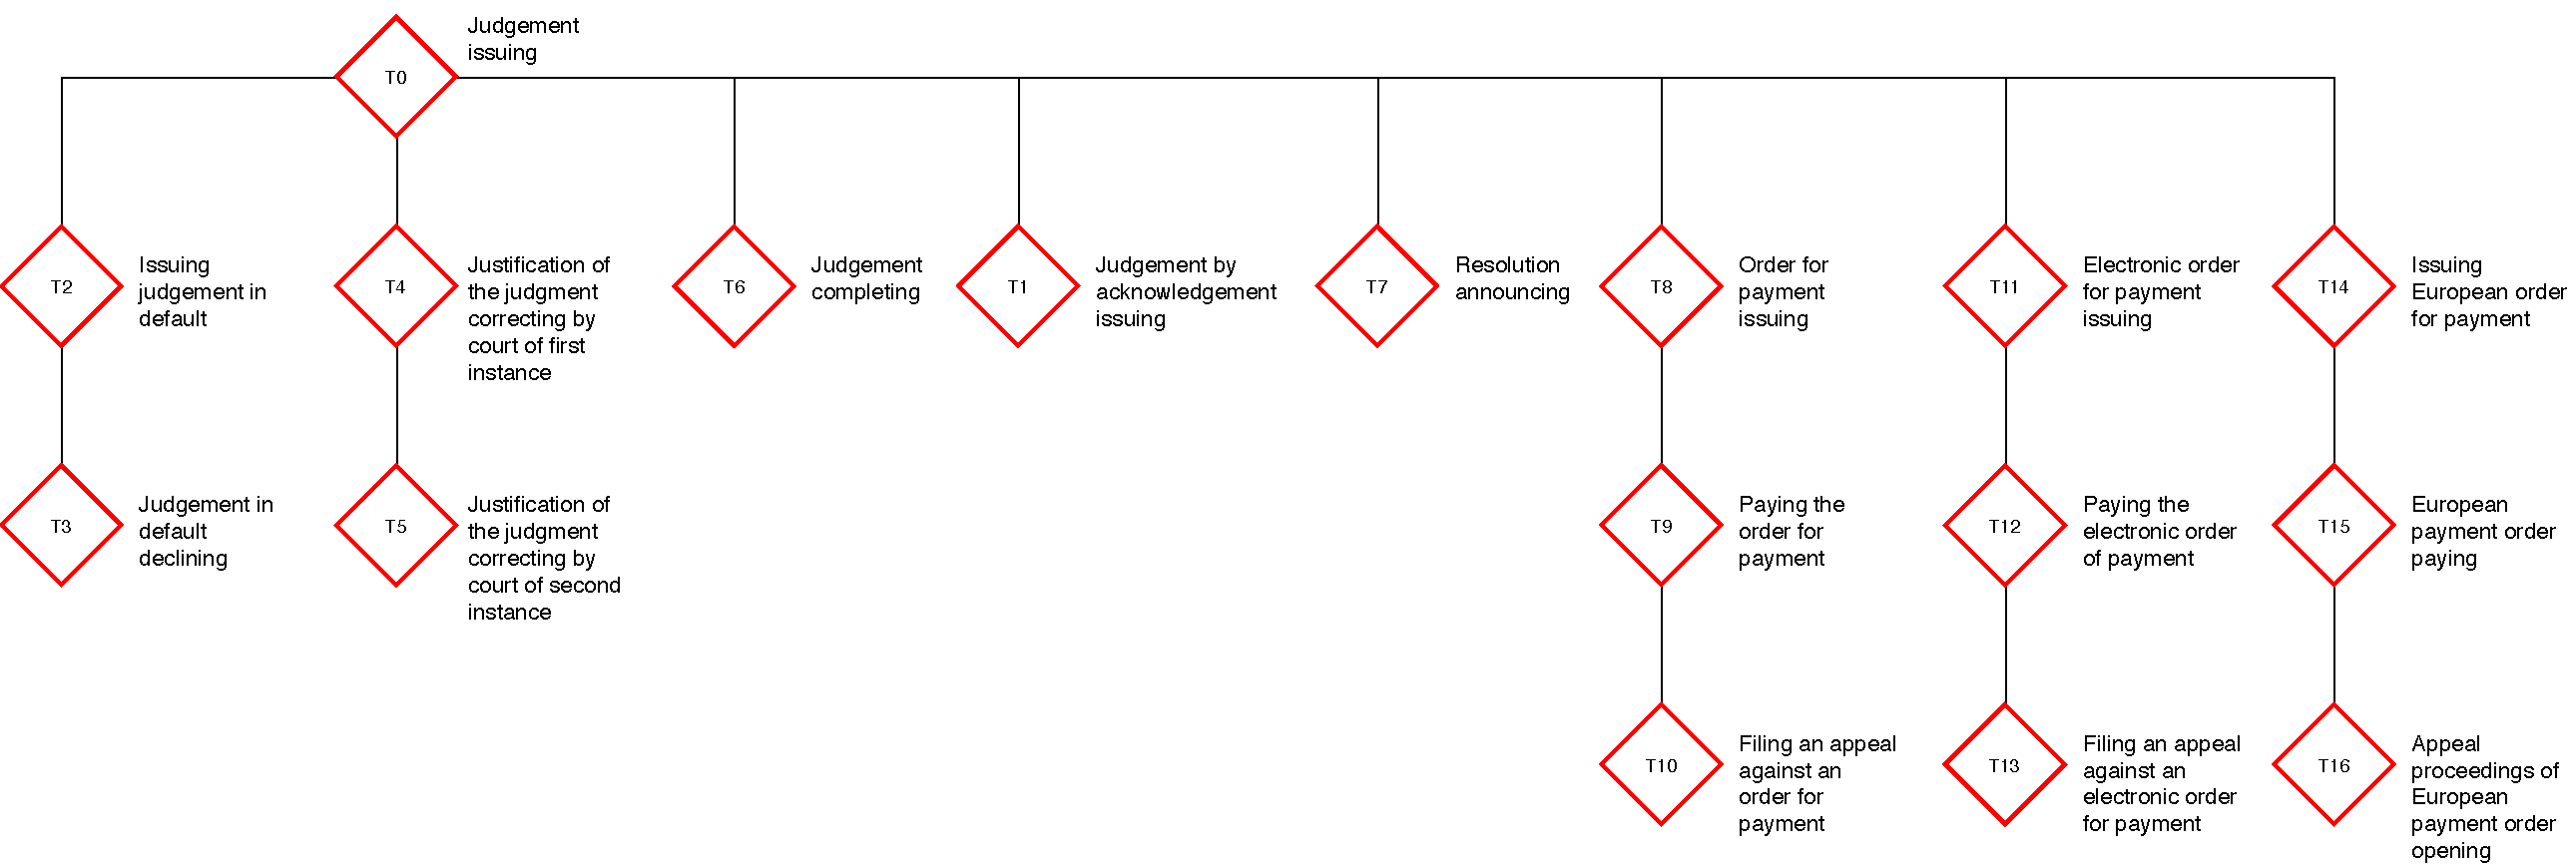
\includegraphics[width=\textwidth]{pic/tree}
	\caption{Interaction Structure Model}
	\label{fig:interactionStructure}
\end{figure}

\begin{figure}[h]\centering
	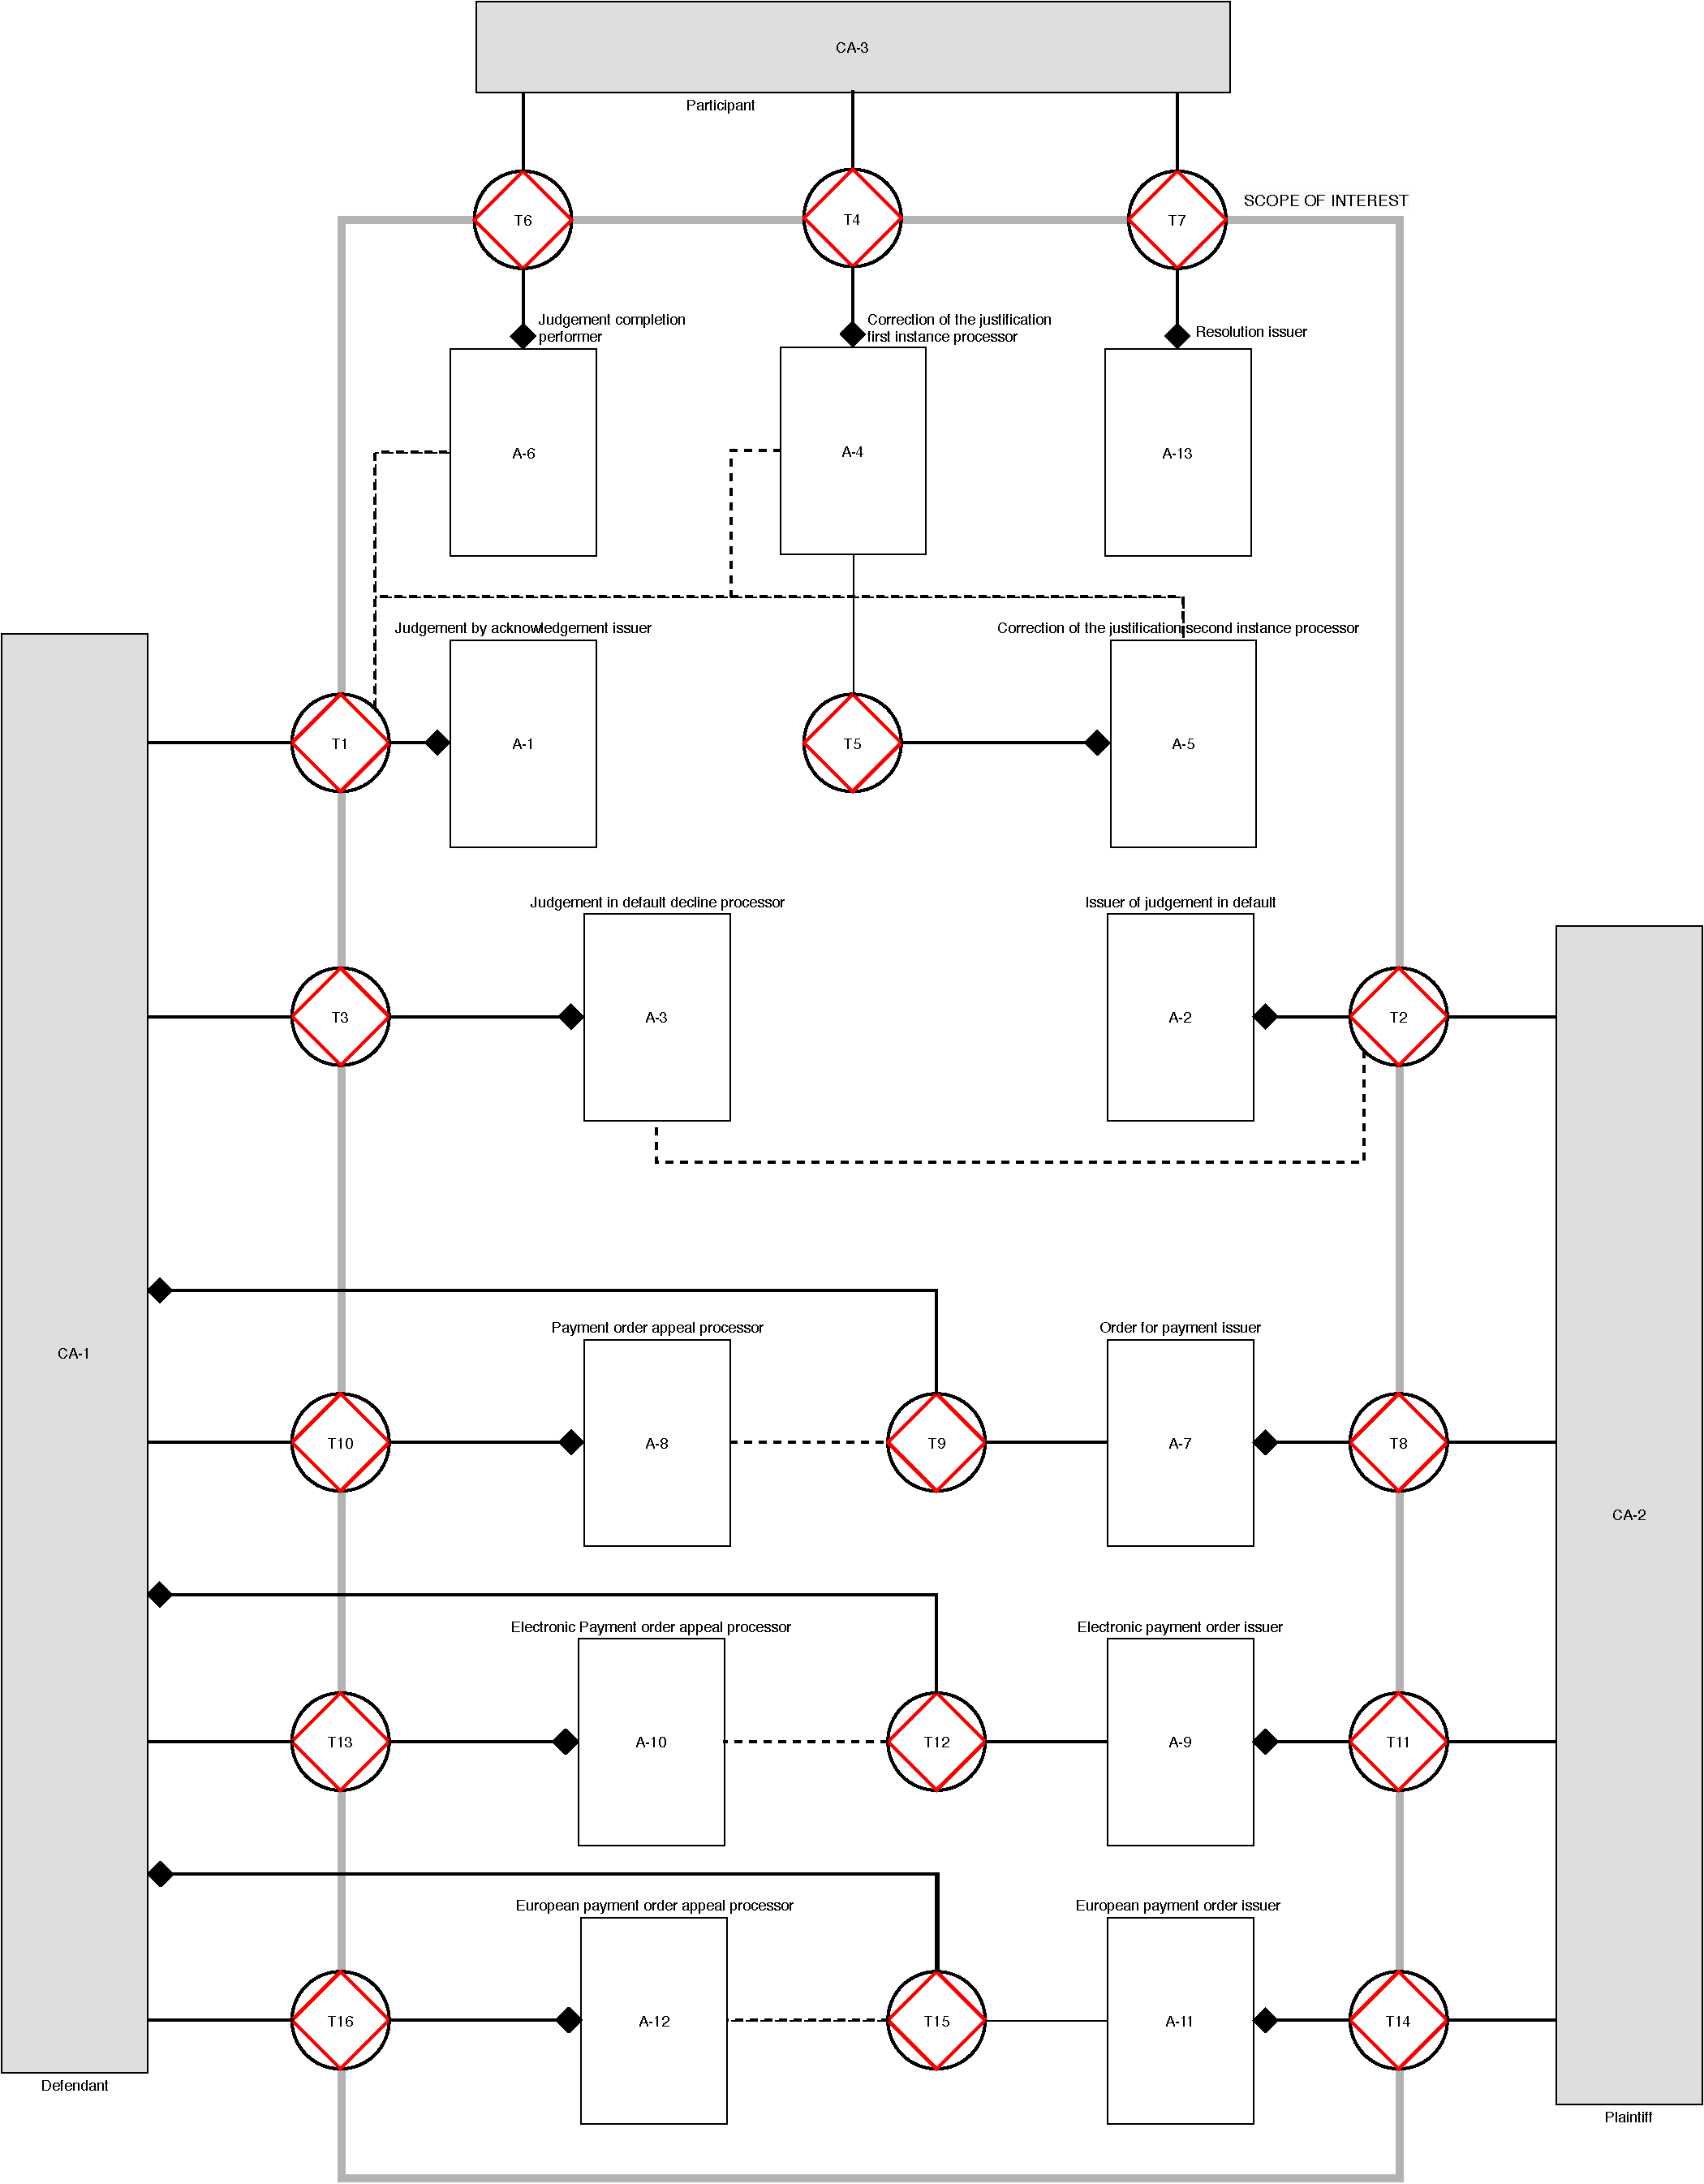
\includegraphics[width=\textwidth]{pic/ocd}
	\caption{An OCD Model}
	\label{fig:csdModel}
\end{figure}

\begin{figure}[h]\centering
	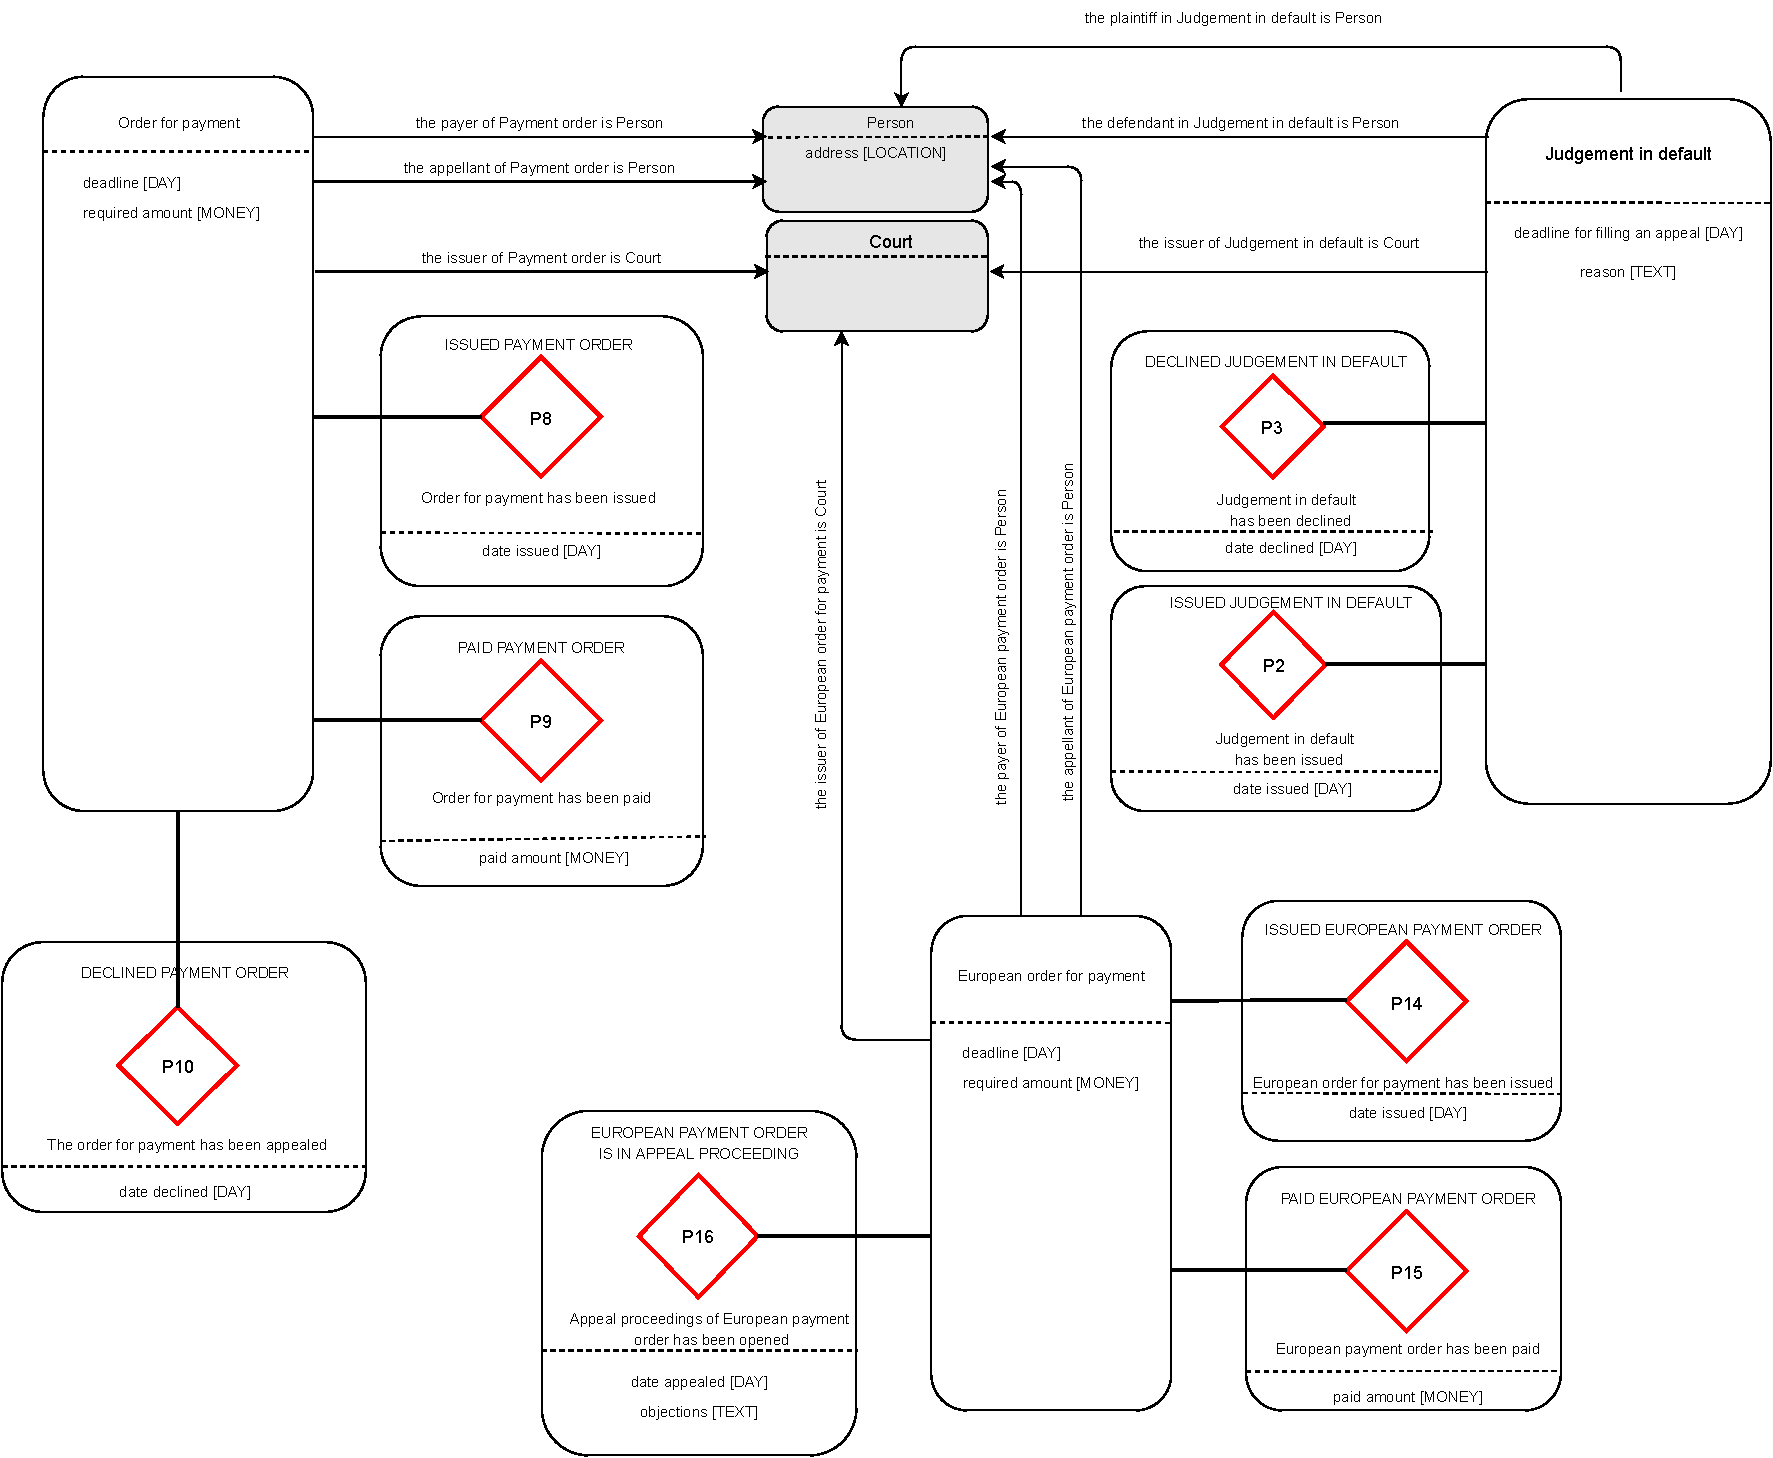
\includegraphics[width=\textwidth]{pic/ofd}
	\caption{An Object Fact Diagram}
	\label{fig:ofdModel}
\end{figure}

\section{Summary}

Some comments about the OER analysis belong here. Why were you not able find some responsibilities? What was vaguely defined? Just roast the authors of the assignment (not the teachers :). 

And finally, show how much information is missing in a table~\cref{tab:missing_transaction_steps}. 

\begin{table}[h]\centering
\caption{Missing Transaction Steps}
\label{tab:missing_transaction_steps}
\begin{tabular}{|l||l|l|l|}
\hline
                      & Specified    & Not Specified & Missing Information \\ \hline
\multicolumn{4}{|c|}{Standard Transaction Pattern}                        \\ \hline
Request               & 14           & 2            & 12,5\%             \\ \hline
Promise               & 0           & 16           & 100\%            \\ \hline
Decline               & 13          & 3           & 18,75\%             \\ \hline
Declare               & 14           & 2            & 12,5\%              \\ \hline
Reject                & 0            & 16           & 100\%             \\ \hline
Accept                & 0           & 16            & 100\%            \\ \hline
\textbf{Total}        & \textbf{41} & \textbf{55}  & \textbf{57,3\%}   \\ \hline
\multicolumn{4}{|c|}{Revokes}                                             \\ \hline
Revoke Request        & 3            & 13           & 81,25\%             \\ \hline
Revoke Promise        & 0            & 16           & 100\%             \\ \hline
Revoke Declare        & 0            & 16           & 100\%            \\ \hline
Revoke Accept         & 0            & 16           & 100\%             \\ \hline
\textbf{Total}        & \textbf{3}   & \textbf{61} & \textbf{95,3\%}    \\ \hline
\multicolumn{4}{|c|}{Complete Transaction Pattern}                        \\ \hline
\textbf{Total}        & \textbf{44} & \textbf{116} & \textbf{72,5\%}    \\ \hline
\end{tabular}

\end{table}